\documentclass[tikz,border=4pt]{standalone}
\usepackage{amsmath,amssymb}\renewcommand{\familydefault}{\sfdefault}
\usepackage{pgfplots}\pgfplotsset{compat=1.17}
\usetikzlibrary{arrows.meta,positioning,shadows,fit,calc,backgrounds,patterns}
\definecolor{lav}{HTML}{E6E6FF}\definecolor{pinkb}{HTML}{FFDDDD}\definecolor{greenb}{HTML}{DDFFDD}\definecolor{yelb}{HTML}{FFFBCF}\definecolor{peach}{HTML}{FFEBD6}\definecolor{mauve}{HTML}{F0E6F0}
\definecolor{reqblue}{HTML}{0000BB}\definecolor{resgreen}{HTML}{008800}\definecolor{dred}{HTML}{CC0000}\definecolor{domblue}{HTML}{000099}\definecolor{crimson}{HTML}{990033}
\definecolor{tbBlue}{HTML}{1F77B4}\definecolor{tbOrange}{HTML}{FF7F0E}\definecolor{tbGreen}{HTML}{2CA02C}\definecolor{tbRed}{HTML}{D62728}\definecolor{tbPurple}{HTML}{9467BD}\definecolor{tbBrown}{HTML}{8C564B}
\definecolor{barGreen}{HTML}{1B8754}\definecolor{darkGreen}{HTML}{2E7D32}\definecolor{lightBlue}{HTML}{A0C4FF}\definecolor{kRed}{HTML}{DC3545}
\definecolor{accB}{HTML}{3366FF}\definecolor{f1O}{HTML}{FF7F50}\definecolor{aucG}{HTML}{44CC11}
\tikzset{node/.style={draw,rounded corners=2.5pt,thick,align=center},
 req/.style={-{Stealth[length=2.4mm]},thick,reqblue},res/.style={-{Stealth[length=2.4mm]},thick,dashed,resgreen}}
\pgfplotsset{every axis/.append style={tick label style={font=\footnotesize},label style={font=\small},title style={font=\small},legend style={font=\scriptsize,fill=white,fill opacity=.9,text opacity=1,draw=black!25,rounded corners=1pt},
 grid style={dotted,black!35}}}
\begin{document}
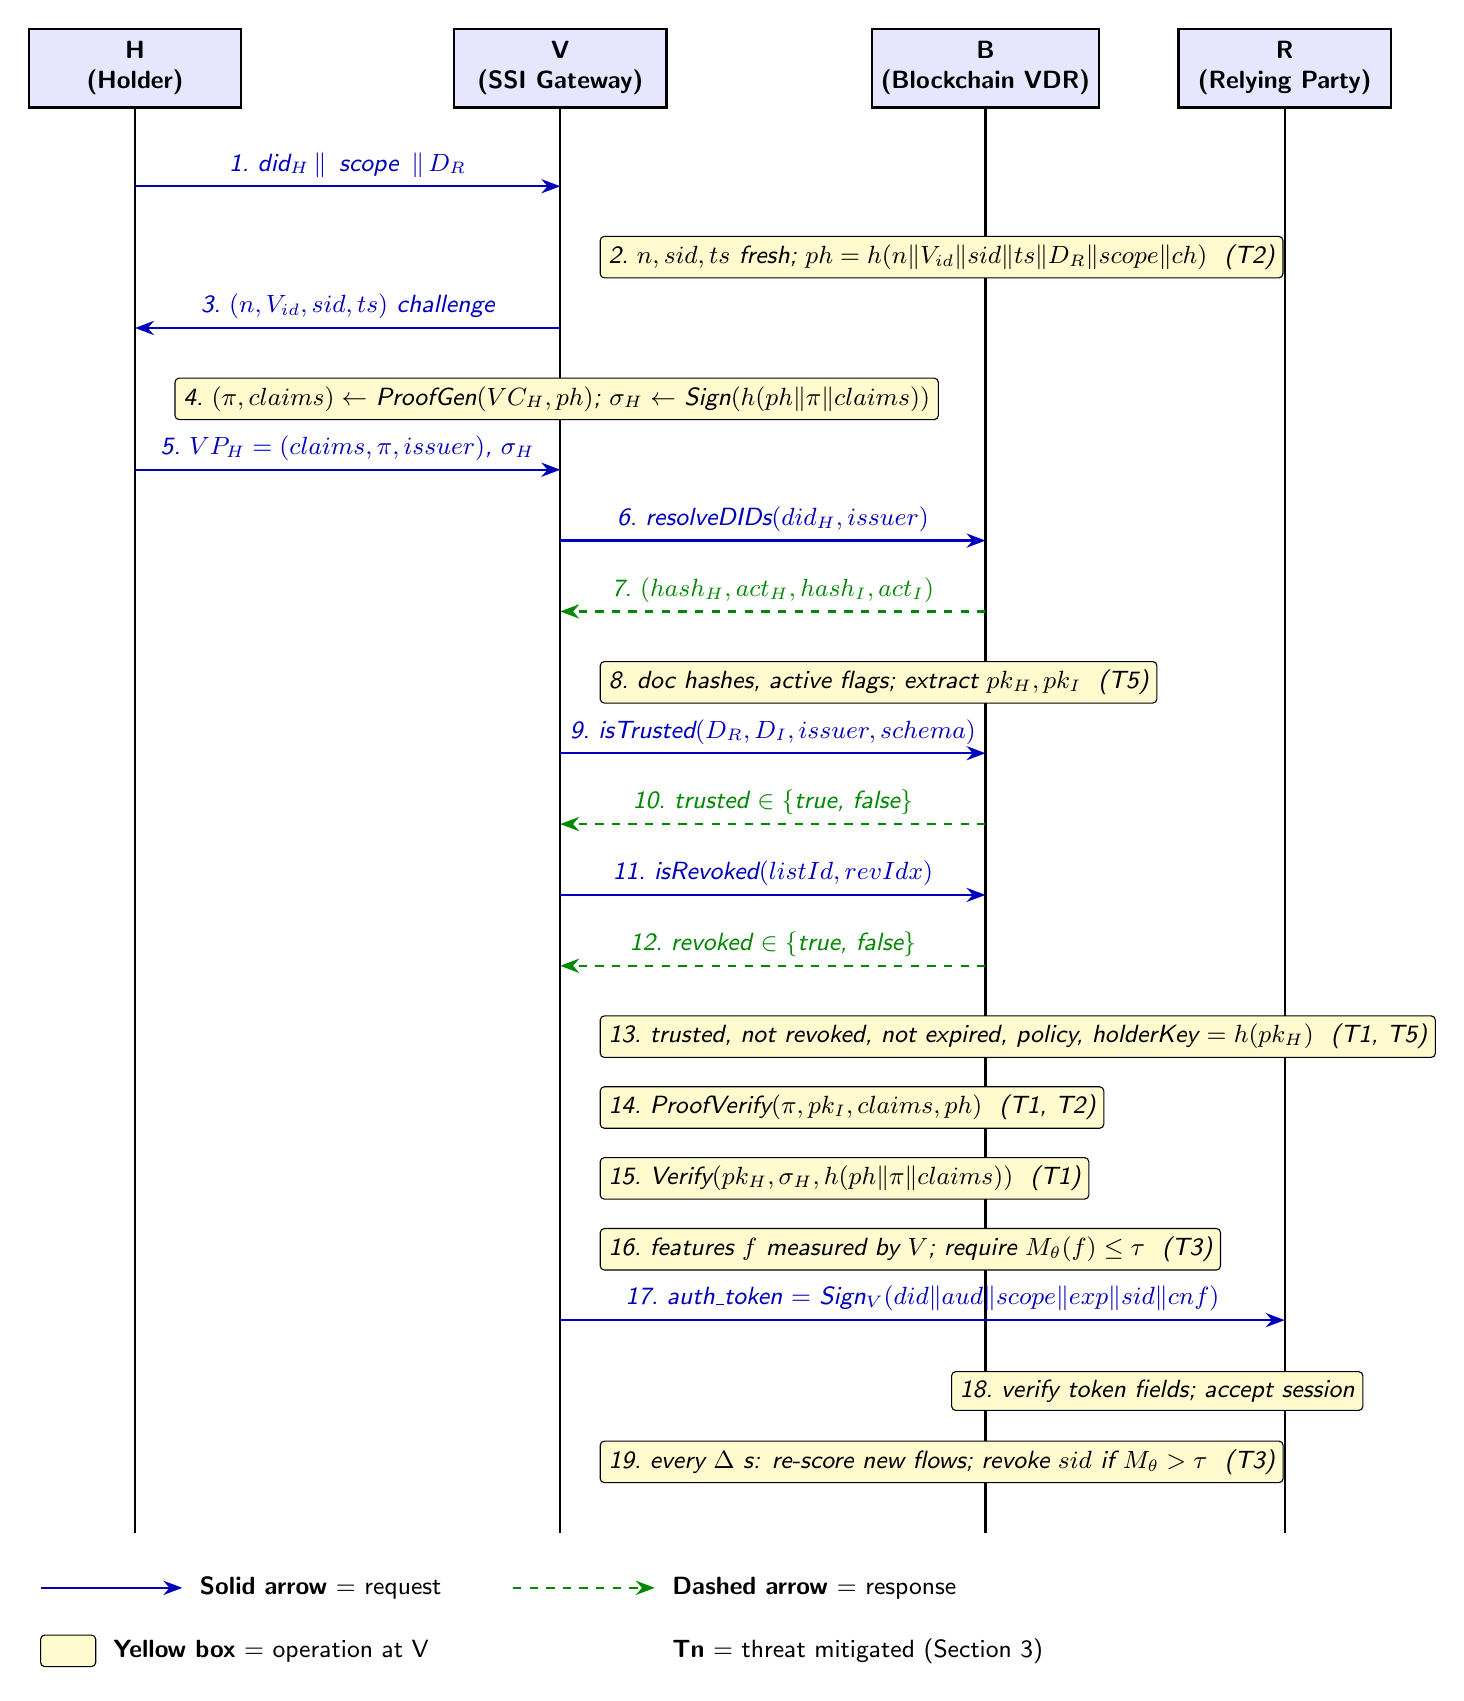
\begin{tikzpicture}[font=\small]
\node[draw,thick,fill=lav,minimum width=2.7cm,minimum height=1.0cm,align=center,font=\small\bfseries] at (0,0) {H\\(Holder)};
\node[draw,thick,fill=lav,minimum width=2.7cm,minimum height=1.0cm,align=center,font=\small\bfseries] at (5.4,0) {V\\(SSI Gateway)};
\node[draw,thick,fill=lav,minimum width=2.7cm,minimum height=1.0cm,align=center,font=\small\bfseries] at (10.8,0) {B\\(Blockchain VDR)};
\node[draw,thick,fill=lav,minimum width=2.7cm,minimum height=1.0cm,align=center,font=\small\bfseries] at (14.6,0) {R\\(Relying Party)};
\draw[thick] (0,-0.5) -- (0,-18.6);
\draw[thick] (5.4,-0.5) -- (5.4,-18.6);
\draw[thick] (10.8,-0.5) -- (10.8,-18.6);
\draw[thick] (14.6,-0.5) -- (14.6,-18.6);
\draw[req] (0,-1.5) -- (5.4,-1.5) node[midway,above=-0.5pt,font=\small\itshape,text=reqblue] {1.\ did$_H \,\|\,$ scope $\,\|\, D_R$};
\node[draw,rounded corners=1.5pt,fill=yelb,anchor=west,font=\small\itshape,inner sep=3pt] at (5.9,-2.4) {2.\ $n, sid, ts$ fresh; $ph = h(n\|V_{id}\|sid\|ts\|D_R\|scope\|ch)$ \ (T2)};
\draw[req] (5.4,-3.3) -- (0,-3.3) node[midway,above=-0.5pt,font=\small\itshape,text=reqblue] {3.\ $(n, V_{id}, sid, ts)$ challenge};
\node[draw,rounded corners=1.5pt,fill=yelb,anchor=west,font=\small\itshape,inner sep=3pt] at (0.5,-4.2) {4.\ $(\pi, claims)\leftarrow$ ProofGen$(VC_H, ph)$;\ $\sigma_H\leftarrow$ Sign$(h(ph\|\pi\|claims))$};
\draw[req] (0,-5.1) -- (5.4,-5.1) node[midway,above=-0.5pt,font=\small\itshape,text=reqblue] {5.\ $VP_H=(claims,\pi,issuer)$, $\sigma_H$};
\draw[req] (5.4,-6.0) -- (10.8,-6.0) node[midway,above=-0.5pt,font=\small\itshape,text=reqblue] {6.\ resolveDIDs$(did_H, issuer)$};
\draw[res] (10.8,-6.9) -- (5.4,-6.9) node[midway,above=-0.5pt,font=\small\itshape,text=resgreen] {7.\ $(hash_H, act_H, hash_I, act_I)$};
\node[draw,rounded corners=1.5pt,fill=yelb,anchor=west,font=\small\itshape,inner sep=3pt] at (5.9,-7.8) {8.\ doc hashes, active flags; extract $pk_H, pk_I$ \ (T5)};
\draw[req] (5.4,-8.7) -- (10.8,-8.7) node[midway,above=-0.5pt,font=\small\itshape,text=reqblue] {9.\ isTrusted$(D_R, D_I, issuer, schema)$};
\draw[res] (10.8,-9.6) -- (5.4,-9.6) node[midway,above=-0.5pt,font=\small\itshape,text=resgreen] {10.\ trusted $\in\{$true, false$\}$};
\draw[req] (5.4,-10.5) -- (10.8,-10.5) node[midway,above=-0.5pt,font=\small\itshape,text=reqblue] {11.\ isRevoked$(listId, revIdx)$};
\draw[res] (10.8,-11.4) -- (5.4,-11.4) node[midway,above=-0.5pt,font=\small\itshape,text=resgreen] {12.\ revoked $\in\{$true, false$\}$};
\node[draw,rounded corners=1.5pt,fill=yelb,anchor=west,font=\small\itshape,inner sep=3pt] at (5.9,-12.3) {13.\ trusted, not revoked, not expired, policy, holderKey $=h(pk_H)$ \ (T1, T5)};
\node[draw,rounded corners=1.5pt,fill=yelb,anchor=west,font=\small\itshape,inner sep=3pt] at (5.9,-13.200000000000001) {14.\ ProofVerify$(\pi, pk_I, claims, ph)$ \ (T1, T2)};
\node[draw,rounded corners=1.5pt,fill=yelb,anchor=west,font=\small\itshape,inner sep=3pt] at (5.9,-14.1) {15.\ Verify$(pk_H, \sigma_H, h(ph\|\pi\|claims))$ \ (T1)};
\node[draw,rounded corners=1.5pt,fill=yelb,anchor=west,font=\small\itshape,inner sep=3pt] at (5.9,-15.0) {16.\ features $f$ measured by $V$; require $M_\theta(f)\le\tau$ \ (T3)};
\draw[req] (5.4,-15.9) -- (14.6,-15.9) node[midway,above=-0.5pt,font=\small\itshape,text=reqblue] {17.\ auth\_token $=$ Sign$_V(did\|aud\|scope\|exp\|sid\|cnf)$};
\node[draw,rounded corners=1.5pt,fill=yelb,anchor=east,font=\small\itshape,inner sep=3pt] at (15.6,-16.8) {18.\ verify token fields; accept session};
\node[draw,rounded corners=1.5pt,fill=yelb,anchor=west,font=\small\itshape,inner sep=3pt] at (5.9,-17.7) {19.\ every $\Delta$ s: re-score new flows; revoke $sid$ if $M_\theta>\tau$ \ (T3)};
\draw[req] (-1.2,-19.3) -- (0.6,-19.3); \node[anchor=west,font=\small] at (0.7,-19.3) {\textbf{Solid arrow} = request};
\draw[res] (4.8,-19.3) -- (6.6,-19.3); \node[anchor=west,font=\small] at (6.7,-19.3) {\textbf{Dashed arrow} = response};
\node[draw,rounded corners=1.5pt,fill=yelb,minimum width=0.7cm,minimum height=0.4cm] at (-0.85,-20.1) {}; \node[anchor=west,font=\small] at (-0.4,-20.1) {\textbf{Yellow box} = operation at V};
\node[anchor=west,font=\small] at (6.7,-20.1) {\textbf{Tn} = threat mitigated (Section 3)};
\end{tikzpicture}
\end{document}